\chapter{Heat MPI parallelization}
%\label{chapter:title}

% Present a speedup graph with the scalability of your MPI application. Show results for resolutions 2000 and 6000. The x-axis is the number of cores and the y-axis the speedup. Use up to four nodes. Add a new node only, when all the physical cores on the already used nodes are busy. Otherwise, we loose efficiency.  Discuss your results.

\section{Ping Pong}

In this task, a simple program was written to send a message from node A to B and back, a so-called ping-pong. The following code snippet shows the main part of the program executing the message passing with blocking send and receive commands.

\begin{lstlisting}[language=C]
double measure_pingpong(const int rank, const int repeats, const int msg_size) {
    int partner_rank = (rank + 1) % 2;

    char *message = (char*)malloc(msg_size);
    memset(message, 'a', msg_size);

    MPI_Barrier(MPI_COMM_WORLD);

    double start_time = 0;
    double end_time = 0;

    start_time = MPI_Wtime();
    for(int _ = 0; _ < repeats; _++){
        if (rank == 0){
            MPI_Send(message, msg_size, MPI_CHAR, partner_rank, 0, MPI_COMM_WORLD);
            MPI_Recv(message, msg_size, MPI_CHAR, partner_rank, 0, MPI_COMM_WORLD, MPI_STATUS_IGNORE);;
        }
        else if (rank == 1){
            MPI_Recv(message, msg_size, MPI_CHAR, partner_rank, 0, MPI_COMM_WORLD, MPI_STATUS_IGNORE);;
            MPI_Send(message, msg_size, MPI_CHAR, partner_rank, 0, MPI_COMM_WORLD);
        }
    }
    end_time = MPI_Wtime();

    free(message);
    return end_time - start_time;
}
\end{lstlisting}

An MPI\_Barrier was enforced before starting measurements to ensure synchronisation. Then, a message of variable size is passed between two MPI processes through MPI\_Send and MPI\_Receive. Finally, the total time the message took to travel between nodes A and B and back is measured and returned to be printed by process 0 in the main function.

Startup time measurement??

The bandwidth of the transfer was measured by repeating the ping pong between two nodes 200 times. The bandwidth could then be calculated through \(bandwidth = (2 \cdot msg\_size \cdot repeats) / total\ time\), where the size of the message (between $2^0$ and $2^{24}$ bytes) was multiplied by the number of measurements, and then divided by the total time. These measurements were done for messages passed between two processing units of one socket, between two sockets of the same node, and across two nodes. The results of these measurements can be seen in \autoref{fig:ex51}. 

\begin{figure}[h]
    \centering
    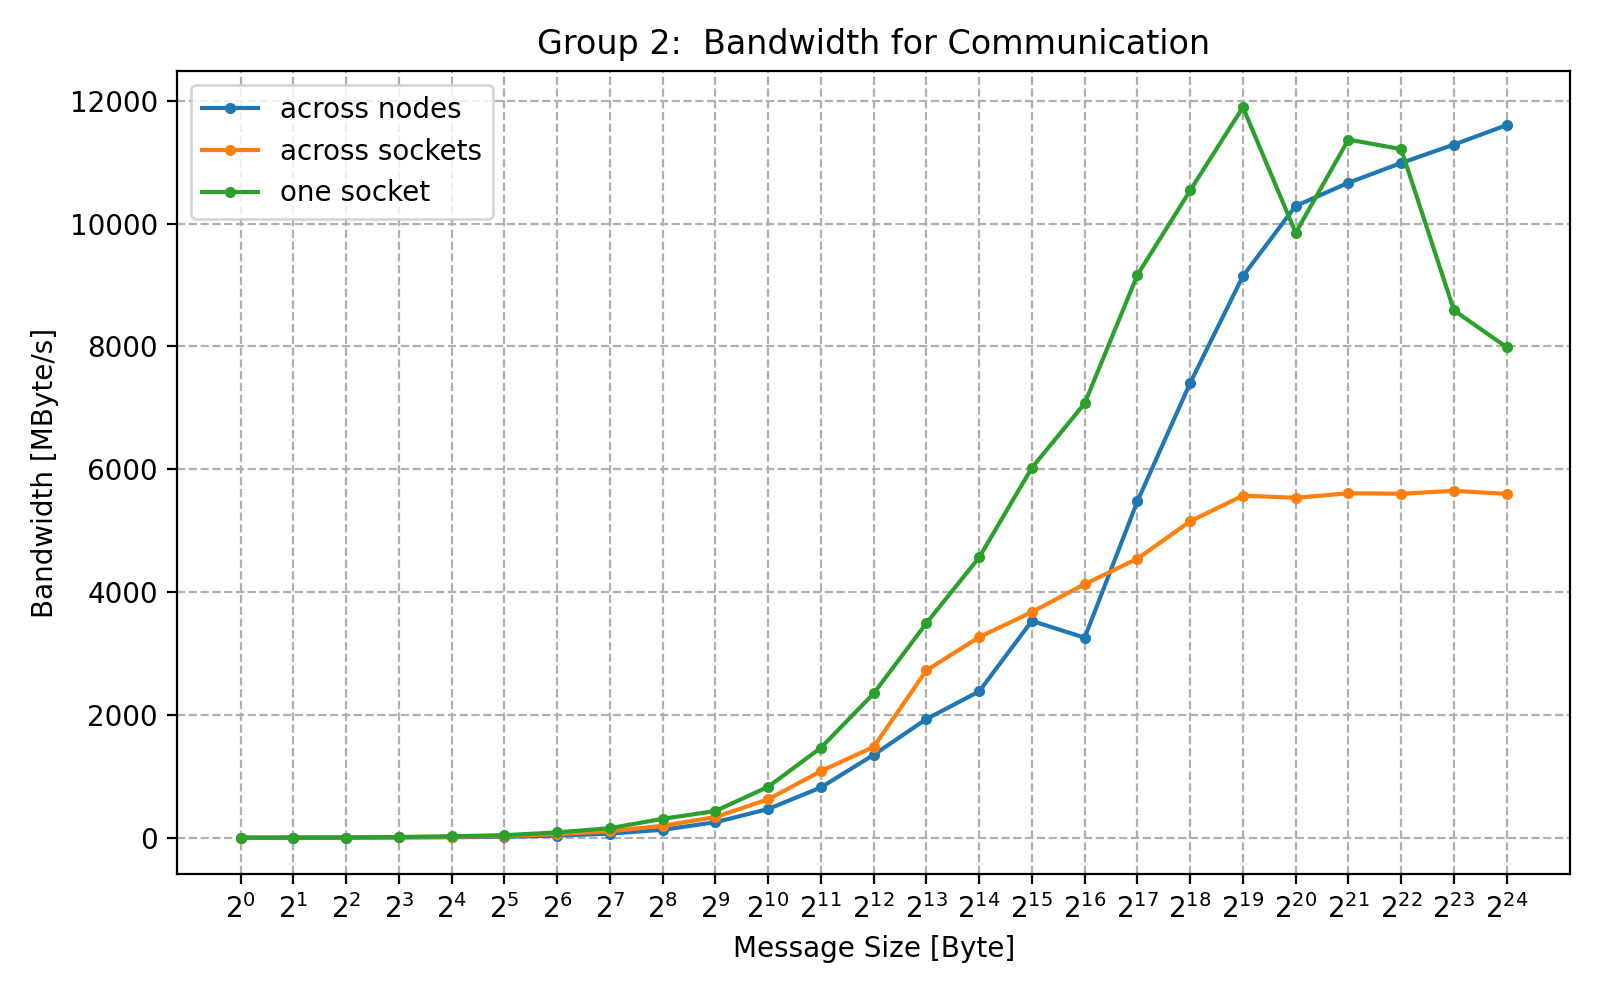
\includegraphics[width=1.0\linewidth]{figures/ex5.png}
    \caption{Communication bandwidth between two nodes on the same socket, across sockets on one node, and across nodes.}
    \label{fig:ex51}
\end{figure}

From this figure it can be seen that there are significant differences in performance between the three different configurations. The maximum bandwidths of each configuration are limited by the different communication protocols used. Between two cores on one socket, there is a kind of "shared memory" as the L3 cache is shared, which makes sending data between the two cores fast. The L3 cache size is 1.3 MB per core, which means a total cache size of around 30 MB. This fits the maximum message size of $2^{24}$ B, or 16 MB, easily. drop at end, cache conflict

The bandwidth between two nodes is clearly limited by the maximum bandwidth of the OmniPath interconnect, which is 100 GB/s.

The maximum bandwidth achieved between two nodes on different sockets of one node is significantly lower than for the other two configurations. Communication between sockets goes through UPI, which has a maximum bandwidth of 25.6 GB/s. Double channel, what conclusion to draw

Eager threshold discussion

Cache coherency?






% Determine
% \begin{itemize}
%   \item the startup time is the time spent to inject and extract a message to and from the network. 
%   \item the bandwidth (MB/s), that is the size of the message in bytes divided by the time for messages of length 20, 21 -224 bytes.
% \end{itemize}
% Synchronize all processes at the beginning by a barrier. To get around measurement inaccuracies, send the message multiple times and measure the aggregated time.


% Perform the measurement for 
% \begin{itemize}
%   \item communication of processes in the same processor,
%   \item same socket but different processors,
%   \item and for processes on different sockets. 
% \end{itemize}



\section{Reduction}

In this task, a program to calculate the reductive sum of an array using a tree structure was created. No MPI collective operations were used. The number of processors was assumed to be a power of 2. The following code snippet shows the program.

\begin{lstlisting}[language=C]
#include <stdio.h>
#include <stdlib.h>
#include <mpi.h>

int RANK = -1;
int SIZE = -1;

/*
 * Get ARRAY_SIZE env variable, if defined, otherwise returns 0.
*/
size_t get_array_size() {
    size_t array_size = 0;
    char *envValue = getenv("ARRAY_SIZE");
    if (envValue != NULL) {
        array_size = atoi(envValue);
        if (array_size == 0)
            printf("ARRAY_SIZE is %d\n", array_size);
    } else {
        if (array_size == 0)
            printf("ARRAY_SIZE environment variable is not set, default is %d.\n", array_size);
	}
    return array_size;
}

/*
 * Initializes and return sum or array.
 */
int set_local_array(int* local_array, int local_size, int start_value) {
    int local_sum = 0; 
    for (int i = 0; i < local_size; i++) {
        local_array[i] = start_value + i;
        local_sum += start_value + i;
    }
    return local_sum;
}

/*
 * Example for 8 processes:
 *  0        1        2        3        4        5        6        7
 *  \       /         \       /         \       /         \       /
 *  0:(0 + 1)          2:(2 + 3)         4:(4 + 5)         6:(6 + 7)
 *      \                /                  \                /
 *       0:(0 + 1 + 2 + 3)                   4:(4 + 5 + 6 + 7)
 *               \                                   /
 *                 0:(0 + 1 + 2 + 3 + 4 + 5 + 6 + 7)
 *  Slash / represent: send to process to the left in the tree, which receives and sums up.
 */
void reduce_and_print_sum(int local_sum) {
    for (int step = 1; step < SIZE; step *= 2) {
        // Processes on the left receive from the right (From those that didn't send
        // in the previous step already; those where stoped with break after send.)
        if (RANK % (2 * step) == 0) {
            int received_sum;
            int source = RANK + step;
            MPI_Recv(&received_sum, 1, MPI_INT, source, 0, MPI_COMM_WORLD, MPI_STATUS_IGNORE);
            local_sum += received_sum;
        } else {
            int target = RANK - step;
            MPI_Send(&local_sum, 1, MPI_INT, target, 0, MPI_COMM_WORLD);
            // Process that sends, is done.
            break;
        }
    }

    if (RANK == 0) {
        printf("Rank %d: Global sum = %d\n", RANK, local_sum);
    }
}

int main(int argc, char *argv[]) {

    size_t array_size = get_array_size();

    MPI_Init(&argc, &argv);
    MPI_Comm_rank(MPI_COMM_WORLD, &RANK);
    MPI_Comm_size(MPI_COMM_WORLD, &SIZE);

    int local_array_size = array_size / SIZE + (RANK < array_size % SIZE);
    int start_value = RANK * (array_size / SIZE) + ((RANK < array_size % SIZE) ? RANK : array_size % SIZE);
    int* local_array = (int *)malloc(local_array_size * sizeof(int));    
    int local_sum = set_local_array(local_array, local_array_size, start_value);

    reduce_and_print_sum(local_sum);

    free(local_array);
    MPI_Finalize();
    return 0;
}
\end{lstlisting}

In this program, the array is first distributed between the different MPI processes. The array is split by dividing it by the number of processes, and then distributing the remainder in a round-robin fashion between the processes starting from process 0. Then, each process calculates a local sum and sends it to its left neighbour in the tree. This procedure is then repeated until all local sums have been sent to process 0, which then combines them and prints the final sum. The process is visualised by comments on lines 38-46 of the code snippet above.

Discussion about tree vs other structures?